%
%  $Description: Author guidelines and sample document in LaTeX 2.09/2e$ 
%
%  $Author: ienne $
%  $Date: 1995/09/15 15:20:59 $
%  $Revision: 1.4 $
%

% \documentstyle[times,twocolumn,latex8]{article} % LaTeX 2.09

\documentclass[10pt,twocolumn]{article}          % LaTeX 2e 
\usepackage{latex8}                              % LaTeX 2e 
\usepackage{times}                               % LaTeX 2e 
\usepackage{graphicx}
\usepackage{cite}
\usepackage{times}
\usepackage[utf8]{inputenc} % this is needed for umlauts
\usepackage[ngerman]{babel} % this is needed for umlauts
\usepackage[T1]{fontenc}    % this is needed for correct output of umlauts in pdf

%------------------------------------------------------------------------- 
% take the % away on next line to produce the final camera-ready version 
%\pagestyle{empty}

%------------------------------------------------------------------------- 
\begin{document}

\title{GPU Computing}

\author{Christian M\"osl\\
University of Salzburg \\ 5020 Salzburg, Austria \\ cmoesl@cs.uni-salzburg.at\\
}

\maketitle
\thispagestyle{empty}

\begin{abstract}
GPU Computing zieht starkes Interesse auf sich, seit dem Machine Learning einen wahnsinnigen Boom erf\"ahrt. 
In dieser Arbeit wird die Geschichte von GPU Computing erkl\"art und welche Probleme gel\"ost werden.
\end{abstract}

\section{Einf\"uhrung}
GPU Computing ist 2020 ist in der Informatik ein sehr gefragtes Thema, vorallem weil unter anderem durch Machine Learning ein grosser Leistungsbedarf da ist.
Die Graphics Processing Unit (GPU) war aber nicht von Anfang an daf\"ur f\"ur diese Aufgabe bestimmt. 
Es hat sich im Laufe der Zeit herausgestellt, dass die Architektur einer GPU sehr vorteilhaft ist und das Berechnen von großen Datenmengen stark beschleunigen kann.
Dies ist vorallem auf die einfache parallelisierbarkeit dieser Probleme zur\"uckzuf\"uhren und der Auslegung der Archtitektur auf m\"oglich viel Datendurchsatz. 


% Introduction,Exact formulation of the problem,Exact formulation of the solution,Correctness considerations (if applicable),Implementation (if applicable),Experimental results and discussion (if any),Conclusion,Acknowledgments.

\section{Geschichte}
Die urspr\"ungliche Aufgabe einer Grafikkarte war es noch, Daten welche im Hauptspeicher des Systems liegen irgendwie in elektrische Signale umzuwandeln, welche dann an den Monitor gesendet werden k\"onnen. 
Das musste auch bei PC Systemen in den 1960er Jahren bereits 60 mal in der Minute durchgef\"uhrt werden. 
Mit dem Aufkommen von immer aufwendigeren Graphical User Interfaces (GUI), wurden Berechnungen f\"ur eben diese bereits von der CPU auf die GPU ausgelagert, sodass die Grafikkarte schließlich zum 2D Beschleuniger wurde.
Die Architektur dieser GPU's war noch auf wenige Befehle eingeschr\"angt und wenig flexibel.
Den wirklichen Ausl\"oser f\"ur den Boom im Grafikkartenmarkt brachten aber vor allem 3D Spiele. \cite{conf}
Das zugrundeliegende Problem hierbei ist hierbei das Rendering einer virtuellen 3D Welt auf einen 2D Monitor.
Hierbei m\"ussen Objekte geometrisch richtig in einen 3D Raum eingef\"ugt werden, was \"uber verschiedene Vektoren beschrieben wird. 
Zus\"atzlich muss noch die Oberfl\"achenstruktur (Textur), Lichtquellen, Schatten und die Perspektive des Betrachters mit ein bezogen werden.
Bei hochaufl\"osenden Texturen ist das nat\"urlich wahnsinnig aufwendig zu berechnen.
Noch versch\"arft wird diese Situation dadurch, dass in Spielen diese Szenen 60 mal in der Sekunde berechnet werden m\"ussen um den Echtzeitanforderungen gerecht zu werden.
Deshalb wurde aus dem 2D Beschleuniger dann ganz schnell ein 3D Beschleuniger um diesen Anforderungen gen\"uge zu tragen.
In diesem Stadium war die Recheneinheit bereits viel komplexer und programmierbarer. \cite{tr}
Als Nvidia schließlich das CUDA Framework 2007 ver\"offentlichte war die Zeit von GPU Computing gekommen.
Gepaart mit einer moderneren und flexibleren Architektur konnte man die GPU nun viel leichter f\"ur das Verarbeiten von großen Datenmengen einsetzen.


\section{Parallelit\"at in Hardware}
Die Architektur einer modernen Grafikkarte ist auf hohen Durchsatz ausgelegt. Das heißt es wird prim\"ar darauf wert gelegt, dass viele Daten auf einmal verarbeitet werden. Dabei werden 2 Kernkonzepte umgesetzt. 
In erster Linie wird versucht mehr kleine (einfachere) Kerne parallel laufen zu haben. \cite{col}
Außerdem werden in diesen Kernen m\"oglichst viele Arithmetische Einheiten untergebracht (ALU). 
Diese vereinfachten Kerne (Shader) bauen auf einem anderen Programmiermodel auf. 
Sogenanntes Streamprocessing, bei dem sich zwar der ganze Shader den Instructionstream teilt, jedoch die Datenfragmente andere sind. 
Das schr\"ankt das Programmiermodel massiv ein und ist nicht mit herk\"omlichen CPU Threads vergleichbar.
Hierbei muss allerdings beachtet werden, dass diese Shader nicht nur einfache Single-Instruction-Multiple-Data (SIMD) Befehle untersch\"utzen.
Es wird zum Beispiel auch Branching in Hardware untersch\"utzt.
Damit das effizient umgesetzt werden kann, m\"ussen die Shader mehrere Ausf\"uhrungskontexte speichern k\"onnen und zwischen diesen umschalten k\"onnen um Stalls zu vermeiden.


\section{Unterst\"utze Konzepte}
Nachfolgend wird \"Uberblick daf\"ur gegeben, welche Programmier Methoden/Konzepte von einer GPU unterst\"utzt werden.

\paragraph{Map} Die Map-Operation wendet einfach die angegebene Funktion (den Kernel) auf jedes Element im Stream an. 
Ein einfaches Beispiel ist das Multiplizieren jedes Werts im Stream mit einer Konstanten (Erh\"ohen der Helligkeit eines Bildes). 
Die Map-Operation ist einfach auf der GPU zu implementieren. 
Der Programmierer erzeugt f\"ur jedes Pixel auf dem Bildschirm ein Fragment und wendet auf jedes ein Programm an. 
Der gleich große Ergebniss Stream wird im Ausgabepuffer gespeichert. \cite{art}

\paragraph{Reduce} Einige Berechnungen erfordern die Berechnung eines kleineren Streams (m\"oglicherweise eines Streams von nur einem Element) aus einem gr\"oßeren Stream. 
Dies wird als Reduzierung des Streams bezeichnet. 
Im Allgemeinen kann eine Reduzierung in mehreren Schritten durchgef\"uhrt werden. 
Die Ergebnisse aus dem vorherigen Schritt werden als Eingabe f\"ur den aktuellen Schritt verwendet, und der Bereich, \"uber den die Operation angewendet wird, wird reduziert, bis nur noch ein Stream-Element \"ubrig bleibt.

\paragraph{Stream filtering} Stream filtering ist im Wesentlichen eine ungleichm\"aßige Reduktion. 
Beim Filtern werden Elemente anhand einiger Kriterien aus dem Stream entfernt.

\paragraph{Scan} Die Scan-Operator, auch als parallele Pr\"afixsumme bezeichnet, nimmt einen Vektor (Stream) von Datenelementen und eine (willk\"urliche) assoziative Bin\"arfunktion '+' mit einem Identit\"atselement 'i' auf. 
Wenn die Eingabe $[a_0, a_1, a_2, a_3, \cdots]$ ist, erzeugt ein exklusiver Scan die Ausgabe $[i, a_0, a_0 + a_1, a_0 + a_1 + a_2, \cdots]$ w\"ahrend ein inklusiver Scan die erzeugt Ausgabe $[a_0, a_0 + a_1, a_0 + a_1 + a_2, a_0 + a_1 + a_2 + a_3, \cdots ]$ und erfordert keine Identit\"at. W\"ahrend die Operation auf den ersten Blick von Natur aus seriell erscheint, sind effiziente Parallel-Scan-Algorithmen m\"oglich und wurden auf Grafikprozessoren implementiert. Die Scanoperation wird beispielsweise bei der Quicksortierung und der sp\"arlichen Matrixvektormultiplikation verwendet.

\paragraph{Sort} Die Sortieroperation wandelt eine ungeordnete Menge von Elementen in eine geordnete Menge von Elementen um. 
Die h\"aufigste Implementierung auf GPUs ist die Verwendung der Radix-Sortierung f\"ur Ganzzahl- und Gleitkommadaten sowie der grobk\"ornigen Zusammenf\"uhrungssortierung und der feink\"ornigen Sortiernetzwerke f\"ur allgemein vergleichbare Daten.

\paragraph{Search} Die Suchoperation erm\"oglicht es dem Programmierer, ein bestimmtes Element innerhalb des Streams zu finden oder m\"oglicherweise Nachbarn eines bestimmten Elements zu finden. 
Die GPU wird nicht verwendet, um die Suche nach einem einzelnen Element zu beschleunigen, sondern um mehrere Suchvorg\"ange gleichzeitig auszuf\"uhren. 
Die verwendete Suchmethode ist meistens die bin\"are Suche nach sortierten Elementen.

\paragraph{Datenstrukturen} Auf der GPU k\"onnen verschiedene Datenstrukturen dargestellt werden wie Arrays (dense/sparse) und Union Types.

\section{Optimale Probleme}
Ob ein Problem sich f\"ur GPU Computing eignet h\"angt von der Struktur ab und ob sich das Problem gut Parallel berechnen l\"asst.

\paragraph{Embarrisingly-Parallel}
Zum Gl\"uck sind eine ganze Menge an Problemen ganz einfach parallelisierbar. 
Hierbei lassen sich zum Beispiel die Eingangsdaten einfach partitionieren, wobei dann f\"ur jede Partition ein Ergebniss unabh\"angig von den anderen Partiionen errechnet werden kann.
Beispiele hierf\"ur w\"aren zum Beispiel das Brute-force raten des Eingangswertes einer Einwegfunktion (Passwort cracking). 
Auch im 3D Rendering bei der Verwendung von Ray Tracing ist es ganz einfach nachvollziehbar, dass das Ergebniss mehrere Lichtstrahlen in einer gegebenen Umgebung parallel berechnet werden kann.

\paragraph{Inherently-Serial}
Andererseits gibt es dagegen auch Probleme welche komplett ungeeignet f\"ur das GPU Computing sind.
Zum Beispiel wenn f\"ur das L\"osen eines Problems sehr viel Branching gemacht werden muss. 
Ein Beispiel hierf\"ur w\"are das finden von Nullstellen durch das Newton Verfahren.


\section{GPU Performance}
Die Vorteile aus dieser Architektur lassen sich auch Anhand von Benchmarks eindeutig messen.
Ein Standardbenchmark ist hierbei das Messen der m\"oglichen Floating-Point Opertationen pro Sekunde.

\begin{figure}[h]
  \begin{center}
  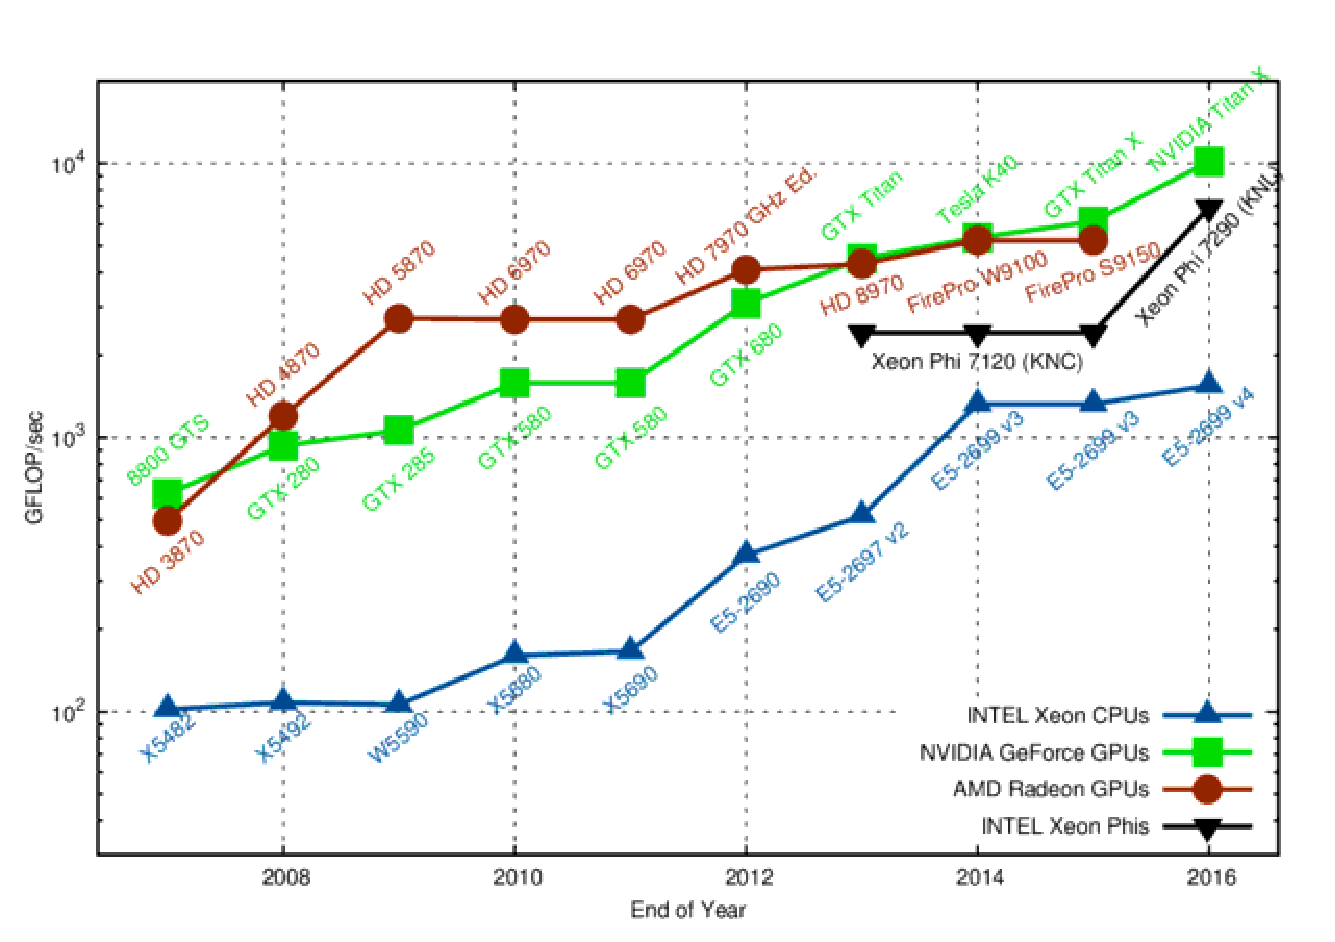
\includegraphics[width=8cm]{gflops.eps}
  \caption{Leistungsunterschied von GPU und CPU}
  \label{fig:flops}
  \end{center}
\end{figure}

Durch die extrem hohe Anzahl an Arithmetischen Recheneinheiten ist hierbei mit einem vielfachen an Leistung gegen\"uber einer herk\"omlichen CPU zu rechnen.
In der Vergangenheit hat sich das auch immer best\"atigt. \ref{fig:flops}

\section{Anwendungsgebiete}
GPU Computing kommt Stand 2020 auch in vielen Anwendungsbereichen auch real zum Einsatz und wird viel genutzt. 

\paragraph{Deep Learning}
Deep Learning steht vereinfacht gesagt f\"ur das Berechnen von Neuronalen Netzen mit vielen/riesigen Schichten.
Eine Schicht besteht aus mehreren Neuronen, wobei jedes Neuron mit jedem anderen Neuron in der n\"achsten Schicht verbunden ist und verrechnet wird.
Beim Training werden nun immer wieder Daten an das Netzwerk angelegt und durch alle Schichten durchgerechnet.
Diese Anwendung eignet sich sehr gut f\"ur GPU Computing, da hier eine große Datenmenge immer nach dem gleichen Schema durchgerechnet wird (Stream Processing).

\section{Fazit}
GPU Computing ist ein sehr popul\"ares und m\"achtiges Tool, das f\"ur viele Anwendungsgebiete geeignet ist. 
Vorallem mit dem Aufkommen von Machine Learning und Big Data ist das ein sehr m\"achtiges Tool um schnelle Datenverarbeitungs Pipelines zu erstellen.
Auch gibt es klare Grenzen, denn nicht jedes Problem l\"asst sich damit schneller Berechnen. 


\nocite{ex1,ex2}
\bibliographystyle{latex8}
\bibliography{main}

\end{document}
